\documentclass[10pt]{beamer}

\usetheme[progressbar=frametitle]{metropolis}
\usepackage{appendixnumberbeamer}
\usepackage{booktabs}
\usepackage[scale=2]{ccicons}
\usepackage{pgfplots}
\usepgfplotslibrary{dateplot}
\usepackage{graphicx}
\usepackage{xspace}
\newcommand{\themename}{\textbf{\textsc{metropolis}}\xspace}

\title{Interactr}
\subtitle{Iteration 3}
\date{\today}
\author{Jelle de Coninck, Hannes De Smet, Bruno Vandekerkhove, Shani Vanlerberghe}
\institute{KULeuven}
% \titlegraphic{\hfill\includegraphics[height=1.5cm]{logo.pdf}}

\begin{document}

\maketitle

\begin{frame}{Table of contents}
  \setbeamertemplate{section in toc}[sections numbered]
  \tableofcontents[hideallsubsections]
\end{frame}

\section{Design}

\begin{frame}[fragile]{Domain Model - Overview}
	\begin{center}
	\begin{itemize}
	\item \texttt{Low representational gap}
	\item Main classes : \texttt{Diagram}, \texttt{Message}, \texttt{Party}
	\item Business logic completely separate from UI
	\end{itemize}
	\end{center}
\end{frame}

\begin{frame}[fragile]{Domain Model - UML}
	\begin{center}
	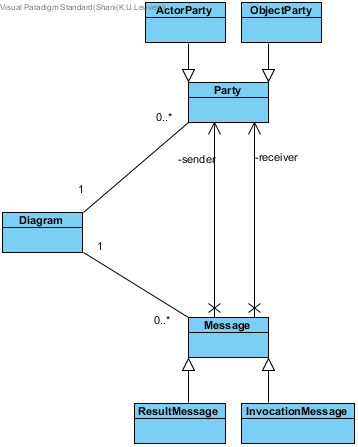
\includegraphics[width=0.6\textwidth]{domain}
	\end{center}
\end{frame}

\begin{frame}[fragile]{Domain Model - Diagram Visitors}
	\begin{center}
	Interface \texttt{DiagramVisitor} can be implemented by various visitors in other subsystems.\\
	Every \texttt{DiagramComponent} can accept such a visitor.\\
	\vspace{0.5cm}
	$\rightarrow$ makes it easy to add functionality to the domain layer without having to add code to the classes themselves (like UI-related code)\\
	\vspace{0.5cm}
	\footnotesize Example of visitors used in our UI layer : \texttt{DialogCreator} (makes dialog for a given diagram component without resorting to the use of \textit{instanceof})
	\end{center}
\end{frame}

\begin{frame}[fragile]{Domain Model - Diagram Observers}
	\begin{center}
	Interface \texttt{DiagramObserver} represents an observer of a diagram. \\
	\vspace{0.5cm}
	A diagram has a list of such observers that it notifies when a party is added, a label is edited, ...\\
	\vspace{0.5cm}
	\footnotesize We currently implement this interface in our classes representing dialog windows and diagram views, for synchronisation of, say, labels.
	\end{center}
\end{frame}

\begin{frame}[fragile]{Entry Point - Controller}
	\begin{center}
	Everything starts in \underline{\texttt{Controller}} :
	\vspace{0.5cm}
	\\$\rightarrow$ creates a \texttt{Window} (extends \texttt{CanvasWindow})
	\\$\rightarrow$ associates the window with \texttt{PaintBoard} (draw events)
	\\$\rightarrow$ associates the window with \texttt{EventHandler} (key/mouse events)
	
	\vspace{0.5cm} Both support \texttt{Protected Variations}. Both encapsulate \textit{awt} package.
	\end{center}
\end{frame}

\begin{frame}[fragile]{Entry Point - Controller}
	\begin{center}
	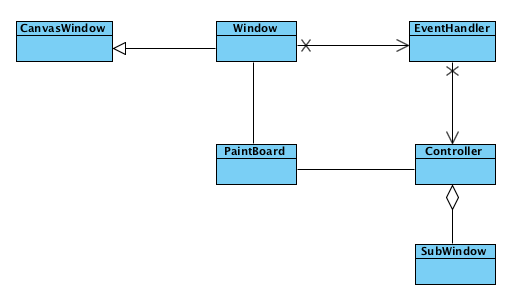
\includegraphics[width=1\textwidth]{entrypoint}
	\end{center}
\end{frame}

\begin{frame}[fragile]{Controller - Underlying Structure}
	\begin{center}
	The \texttt{Controller} keeps track of a list of \texttt{SubWindow}s.
	\\\vspace{0.5cm} A \texttt{SubWindow} can be a \texttt{DiagramWindow} or a \texttt{DialogBox}.
	\\\vspace{0.5cm} Each \texttt{SubWindow} has a frame.
	\\\vspace{0.5cm} \footnotesize Each \texttt{SubWindow} is `\textit{activated}' by putting it at the front of the window list.
	\end{center}
\end{frame}

\begin{frame}[fragile]{SubWindows - Diagram Windows \& Dialog Boxes/Windows}
	\begin{center}
	A \texttt{DiagramWindow} has two \texttt{DiagramView}s.
	\\A \texttt{DialogWindow} aggregates \texttt{Model}s representing \textit{controls}.
	
	\vspace{0.5cm}
	A \texttt{Diagram} is directly altered by \texttt{DiagramView}s and \texttt{DialogWindow}s.
	
	\vspace{0.5cm}
	Synchronization is either done with the \texttt{Observer} pattern, or \textit{lazily} (update upon drawing).
	\\ Since \texttt{Diagram} knows when it changes, it keeps a list of \texttt{DiagramObserver}s and notifies them (\texttt{Information Expert}).
	\\$\rightarrow$ disadvantage : coordinates aren't synchronised (solved by `\textit{making room}' upon addition of a diagram component to a `DiagramView')
	\end{center}
\end{frame}

\begin{frame}[fragile]{Event Handling - How it all Starts}
	\begin{center}
	\begin{itemize}
	\item[$\rightarrow$] Every mouse or key event goes from \texttt{Window} $\rightarrow$ \texttt{EventHandler}.
	\item[$\rightarrow$] \texttt{EventHandler} interprets the events and transforms them into \texttt{Command} instances.
	\item[$\rightarrow$] \texttt{Command} is forwarded to \texttt{Controller}.
	\end{itemize}
	Note : if event is a \textit{mouse press}, \texttt{EventHandler} asks the \texttt{Controller} to activate the \texttt{SubWindow} at that coordinate first. This very window will be the first receiver for the command. 
	\end{center}
\end{frame}

\begin{frame}[fragile]{Event Handling - Commands}
	\begin{center}
	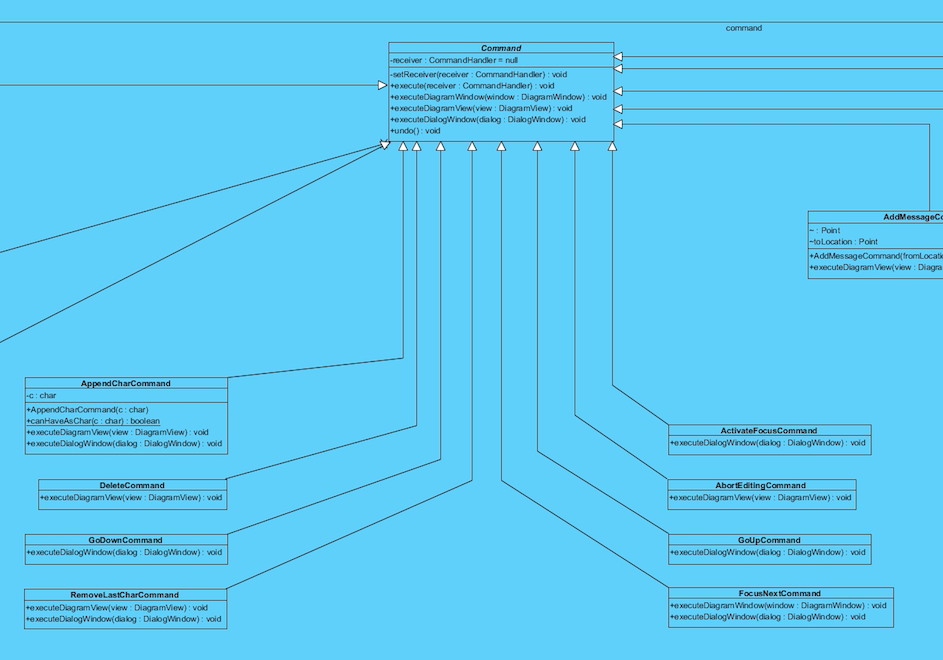
\includegraphics[width=1\textwidth]{command}
	\end{center}
\end{frame}

\begin{frame}[fragile]{Event Handling - Executing Commands}
	\begin{center}
	\textit{Precondition} : \texttt{SubWindow} is active
	\begin{itemize}
	\item[$\rightarrow$] Every \texttt{Command} can be handled by a \texttt{CommandHandler}.
	\item[$\rightarrow$] \texttt{DiagramWindow}, \texttt{DiagramView} and \texttt{DialogBox} extend the \texttt{CommandHandler} class. 
	\item[$\rightarrow$] The first \texttt{CommandHandler} is the active \texttt{SubWindow}.
	\item[$\rightarrow$] Every \texttt{CommandHandler} either deals with the \texttt{Command} or (on failure) passes it to the next \texttt{CommandHandler} in its chain. 
	\end{itemize}
	Patterns used : \texttt{Command}, \texttt{Visitor} and (some sort of) \texttt{Chain of Responsibility}.
	\end{center}
\end{frame}

\begin{frame}[fragile]{Event Handling - Example}
	\begin{center}
	Vid. Sequence diagram for \textit{Add Party}.
	\end{center}
\end{frame}

\begin{frame}[fragile]{Drawing - Paint Board}
	\begin{center}
	The \texttt{PaintBoard} encapsulates the \textit{awt} package. It is passed along to any class responsible for drawing. Drawing is done `\textit{on}' the paint board.
	\begin{itemize}
	\item[-] manages clip rect (to prevent overflowing)
	\item[-] allows color changes
	\item[-] ...
	\end{itemize}
	$\rightarrow$ it is a \texttt{Facade}
	\end{center}
\end{frame}

\begin{frame}[fragile]{Drawing - Displaying Elements}
	\begin{center}
	Each class that displays something draws itself (\texttt{Information Expert}) :
	\begin{itemize}
	\item \texttt{SubWindow} draws title bar, close button, frame.
	\item \texttt{DiagramView} draws diagram with messages, parties, ...
	\\$\rightarrow$ use of \texttt{Visitor} pattern to generate figures (representations) for these diagram components.
	\\$\rightarrow$ these figures are \texttt{Flyweight}s.
	\\$\rightarrow$ separation of UI / domain logic without use of type checking (i.e. \texttt{instanceof}).
	\item Class hierarchy for \texttt{Model} (\texttt{Composite} pattern) used for representation/drawing of a variety of elements in the system (parties, messages, controls, ...).
	\end{itemize}
	\end{center}
\end{frame}

\section{Extensibility}

\begin{frame}[fragile]{Extensibility - Diagram Visitors}
	\begin{center}
		As stated before, \texttt{DiagramVisitor} interface makes it easy to add functionality to the domain model without `polluting' it with, say, UI logic.
	\end{center}
\end{frame}

\begin{frame}[fragile]{Extensibility - Commands}
	\begin{center}
	\texttt{Command} pattern eases undoing, allows delayed processing, use by menu items, ... When using new types of events (eg. speech recognition) only \texttt{EventHandler} has to change.
	
	\vspace{0.5cm} Disadvantages ; 
	\begin{itemize}
	\item many new types of \texttt{CommandHandler}?
	\\ $\rightarrow$ bloated \texttt{Command} abstract class (\texttt{Visitor} pattern discussion)
	\item if \texttt{Chain of Responsibility} is long
	\\ $\rightarrow$ wasted processing (command goes down the whole chain before realising that it can't be handled)
	\item if many new system operations for many different types of windows 
	\\ $\rightarrow$ redesign probably warranted.
	\end{itemize}
	\end{center}
\end{frame}

\begin{frame}[fragile]{Extensibility - Model}
	\begin{center}
	Representation of various elements in the system can be done with the \texttt{Model} class.\\
	$\rightarrow $ new elements in domain model and elsewhere is a matter of creating subclasses of \texttt{Model}, whenever necessary.\\
	\vspace{0.5cm}
	More complex \texttt{Model}s can be made (and recycled) by composing them out of `primitives' (\texttt{Line}s, \texttt{Oval}s, ...).
	\end{center}
\end{frame}

\section{Testing}

\begin{frame}[fragile]{Testing - Coverage}
	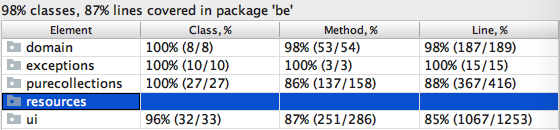
\includegraphics[width=1\textwidth]{coverage}
\end{frame}

\section{Project Management}

%\begin{frame}[fragile]{Management}
%\begin{itemize}
%\item Testing Coordinator : Hannes De Smet
%\item Design Coordinator : Shani Valerberghe
%\item Domain Coordinator
%\end{itemize}
%\end{frame}

\begin{frame}[fragile]{Refactoring}
\begin{itemize}
\item No \textit{duplicated code}.
\item \textit{Moved methods} here and there.
\item Addressed \textit{long methods} with \textit{extract method} \\
$\rightarrow$ not the best metric ... but all methods (easily) `fit on the screen' (max. $\approx$ 25 lines).
\item If appropriate a \textit{temporary variable} was replaced with getters.
\item Avoided \textit{message chains}.
\item Virtually no \textit{switch statements} (in \texttt{EventHandler}).
\item \textit{Comments} never really necessary (maybe when drawing messages in \texttt{SequenceView}).
\end{itemize}
\end{frame}

\begin{frame}[fragile]{Refactoring - Tools}
	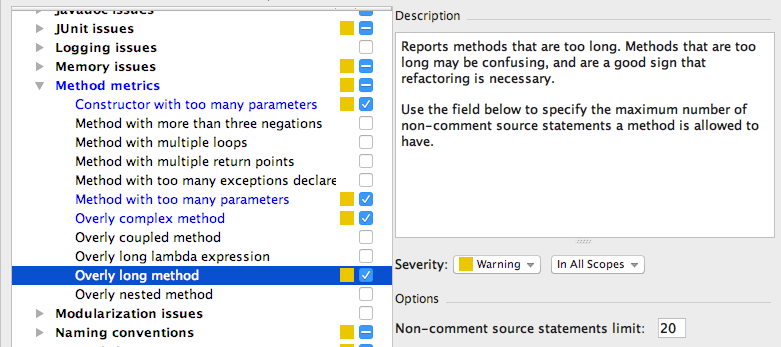
\includegraphics[width=1\textwidth]{refactoring}
\end{frame}

\begin{frame}[fragile]{Time Management}
\begin{itemize}
\item weekly meeting with assistant
\item +- 40 hours per person
\item designed, refactored, tested, redesigned, ... in no particular order
\end{itemize}
\end{frame}

{\setbeamercolor{palette primary}{fg=black, bg=lightgray}
\begin{frame}[standout]
  Demonstration
\end{frame}
}

\end{document}